%!TEX root = TableSummarizationDemo.tex

\section{System Overview}\label{sec:system}

\begin{figure}
\vspace{-5pt}
\centering
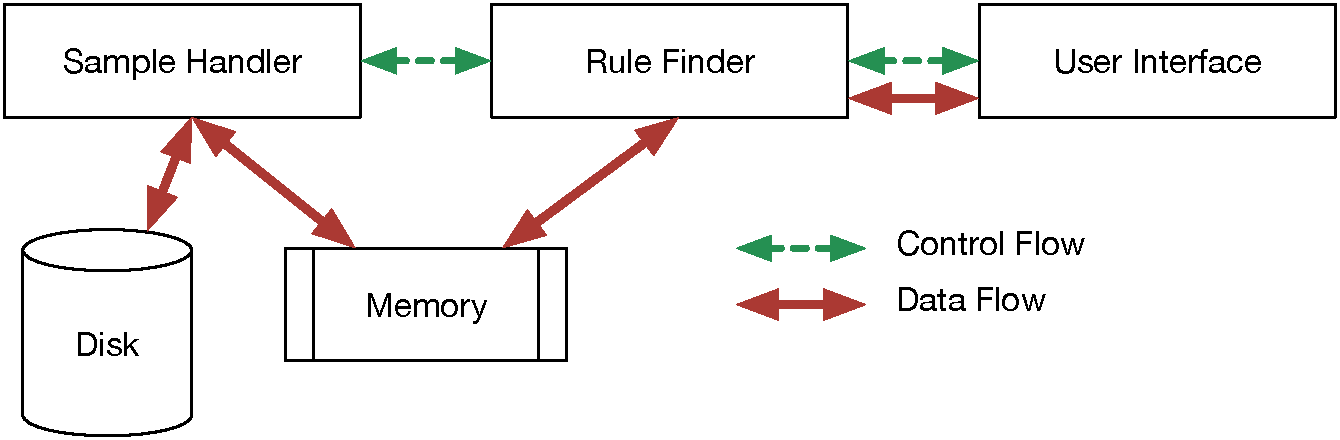
\includegraphics[width=80mm]{graphs/arch.pdf}
\vspace{-20pt}
\caption{The architecture our system \label{fig:system}}
\vspace{-15pt}
\end{figure}

Our system consists of three main components (shown in Figure~\ref{fig:system}): the `Rule Finder', the `Sample Handler' and the `User Interface'. 
At a high level, the User Interface is a web application that allows users to explore
a dataset using smart drill-down. The User Interface invokes the Rule Finder component based on interactions.
The Rule Finder determines what rules to display to a user based on the user's latest interaction, the values of parameters such as number $k$ of rules to display, weighting function $W$ to use, and so on. 
In order to do this, the Rule Finder has to make a pass through the table data several times. This can be expensive for big tables, so we dynamically maintain multiple samples of different parts of the table in memory instead. The Sample Handler is responsible for maintaining samples in memory and updating them when required. 
We now describe the components one by one.

\stitle{Rule Finder.} The problem addressed by the Rule Finder, i.e., that of choosing the optimal rule list of a given size, is NP-Hard. However, we find an approximately optimal solution as follows: We first notice that given a set of rules, a rule-list consisting of those rules has the highest score if the rules are sorted in decreasing order by weight. So we can define the score of a rule {\em set} to be the score of the rule-list obtained by ordering rules of the set in decreasing order by weight. Thus our problem reduces to that of finding the highest scoring rule set. As long as the weight function is monotonic, the score of a rule-set can be shown to be submodular. Then we use the fact that a submodular function can be optimized using a greedy algorithm to choose rules one at a time in a greedy manner until we have $k$ rules. We call the above algorithm BRS (which stands for {\bf B}est {\bf R}ule {\bf S}et). Additional details on our approximation algorithm can be found in our technical report~\cite{tr}. 

\stitle{Sample Handler.} The second component of our system, the `Sample Handler', takes two user-specified input parameters to begin with: the memory capacity $M$, and a parameter called $minSS$. $minSS$ determines the sample size required to run the BRS algorithm. Higher values of $minSS$ increase processing time (since the algorithm has to process a larger amount of data) but also increase the accuracy of the resulting displayed rule-list and rule counts. Then, the Sample Handler maintains a set of samples in memory, such that the sum of sizes of the samples never exceeds $M$. Each sample is a uniformly random subset of tuples that are covered by some rule $r'$. When the user attempts to drill-down on a rule $r$, the Sample Handler appropriately combines tuples from various existing samples to produce a set of at least $minSS$ tuples covered by $r$ to run BRS on. If the Sample Handler cannot create such a set using existing in-memory samples, then it needs to make a pass over the table to generate new samples. In that case, it determines a new set of samples to create, to maximize the probability that the next user click can be responded using those samples. Then it makes a pass through the table to create the new samples. 

%\begin{figure*}[ht]
%\vspace{-5pt}
%\centering
%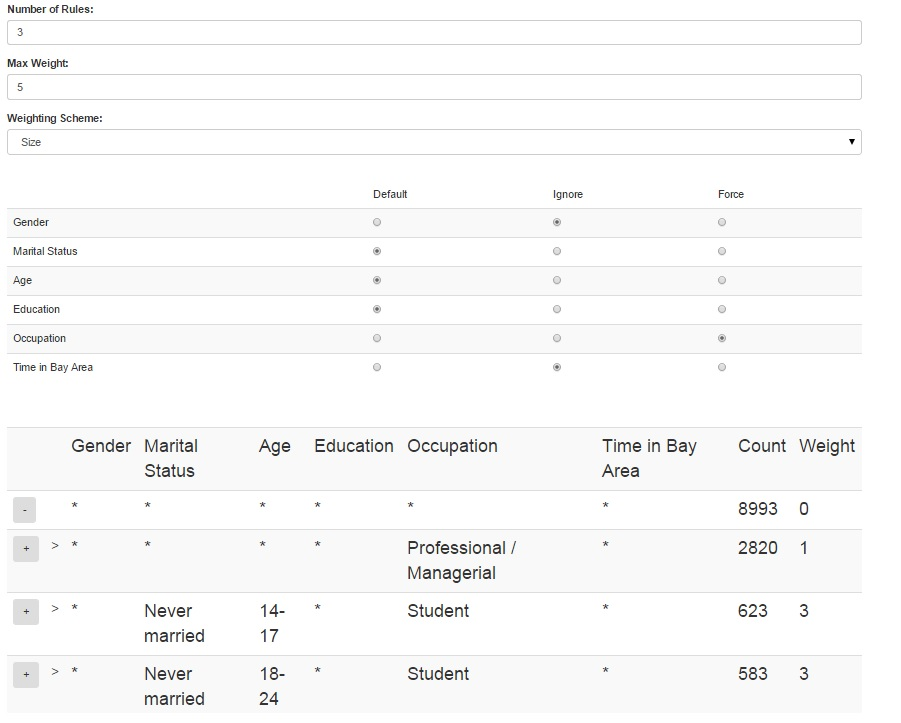
\includegraphics[width=160mm,frame]{graphs/tsapp_screenshot.jpg}
%\vspace{-5pt}
%\caption{The web interface of our system \label{fig:interface}}
%\vspace{-5pt}
%\end{figure*}

\begin{figure}[ht]
\vspace{-5pt}
\centering
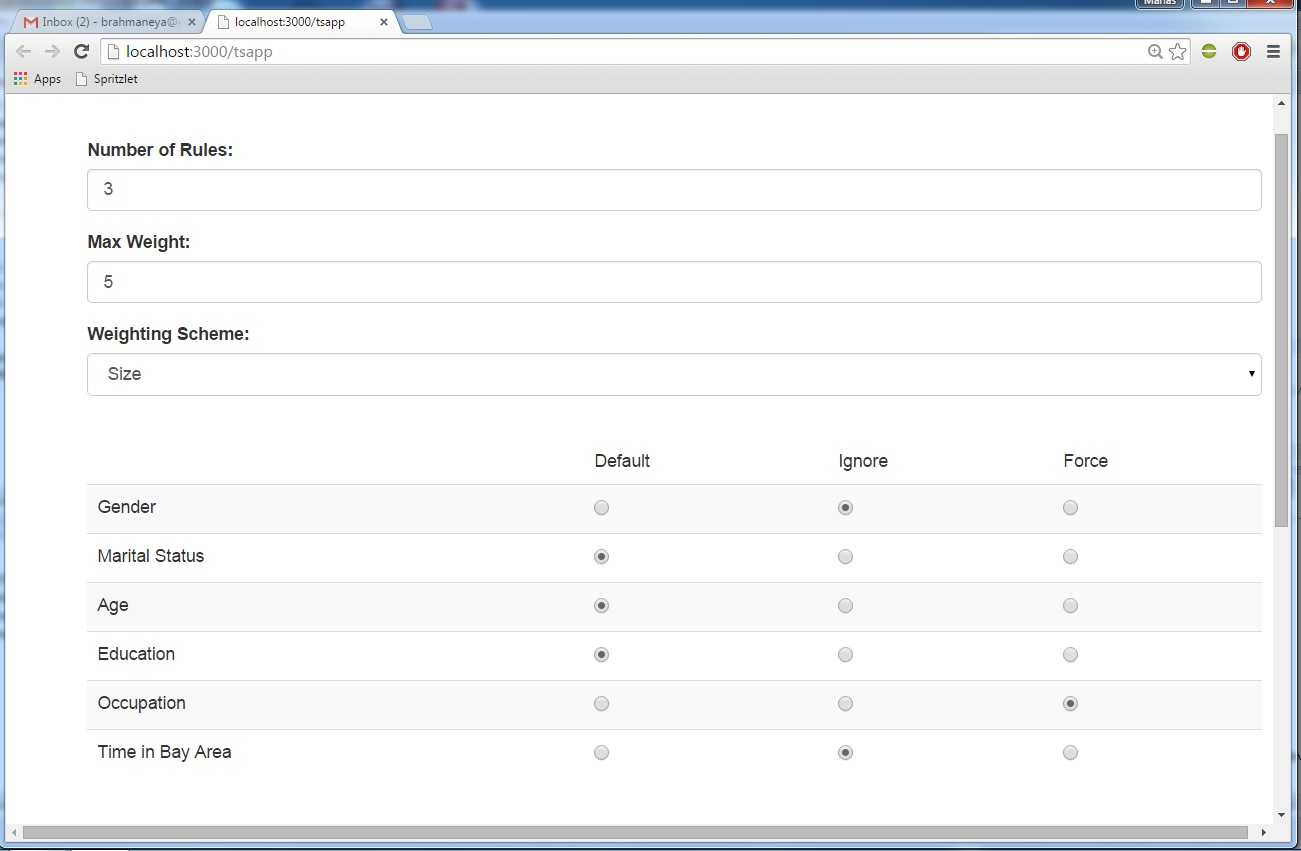
\includegraphics[width=80mm,frame]{graphs/uiscreenshot.jpg}
\vspace{-5pt}
\caption{The web interface of our system: specification of parameters \label{fig:interface}}
\vspace{-5pt}
\end{figure}

\begin{figure}[ht]
\vspace{-5pt}
\centering
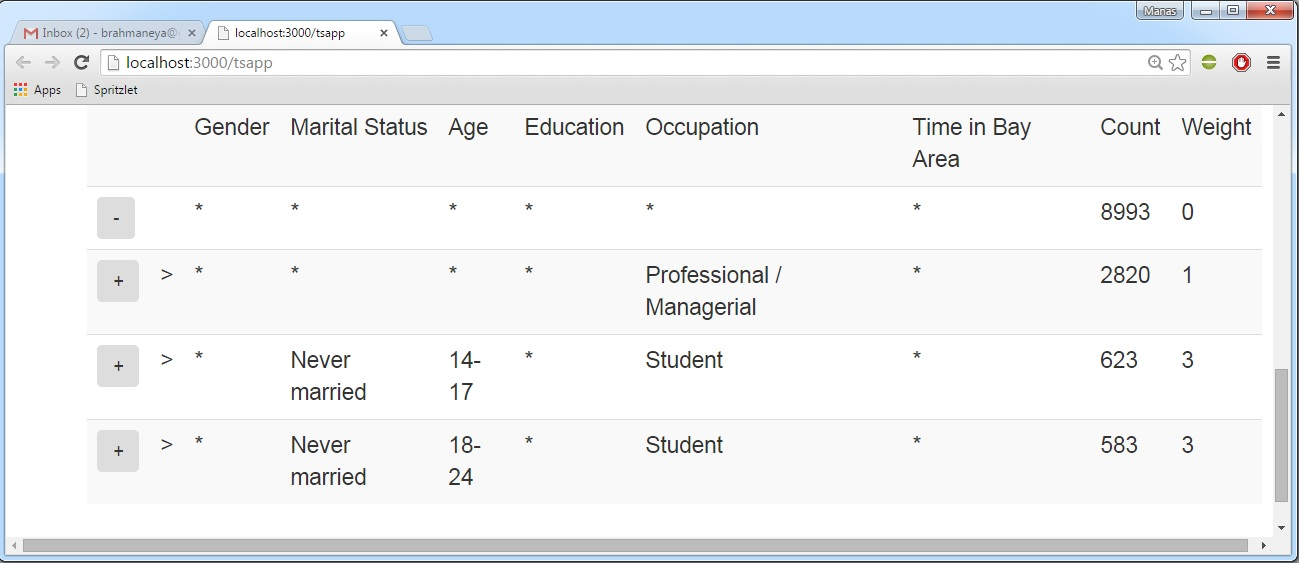
\includegraphics[width=80mm,frame]{graphs/uiresults.jpg}
\vspace{-5pt}
\caption{The web interface of our system: interactive results pane \label{fig:results}}
\vspace{-5pt}
\end{figure}

\stitle{User Interface.} The third component is the User Interface, 
shown in Figure~\ref{fig:interface}, with the results displayed in Figure~\ref{fig:results}.
At the top of the interface in Figure~\ref{fig:interface}, users can set the number 
of new rules to display in response to every smart drill-down. 

The second and third parameters manage weights, which as discussed in Section~\ref{sec:formal} allow a user to modify the interpretation of ``interesting tuples''.
The weighting function (set by the third parameter) is used to specify the importance of a rule, e.g., based on the number of distinct values or the value of particular attributes. In general, our approximation algorithm works for any monotonic weighting function. 
But for ease of use of the web interface, we have hard-coded a few different weighting functions, that can be selected using the drop-down list in the interface.

The second setting, a parameter called max weight, lets the system ignore rules that have high weight (above max weight). The idea behind this is that rules with high weight have a high number of non-$\star$ values, and hence a much smaller Count, making them unlikely to appear in an optimal rule-list. As max weight decreases, rule selection becomes more efficient. As long as the weight of all rules in the optimal rule-list is less than this
parameter, our system displays the optimal rule-list, so there is no impact on the user. However, if max weight is smaller than the weight of some optimal rules, then the user sees an non-optimal set of rules.

Below the drop down menu, the interface displays the set of columns of the database table being explored. Each column has three options: `Default', `Ignore', and `Force'. Choosing the Ignore option causes the column to be ignored, (so the weight given to a rule with a value in that column is set to that of a rule with a $\star$ value in that column). Choosing the Force option forces every displayed rule to have a non-$\star$ value in that column. This is especially useful for tables with a large number of columns, where the user may only be interested in some of the columns. 

Finally, the actual interactive table summary is displayed in Figure~\ref{fig:results}. The plus and minus buttons before the rules can be used to drill-down and reverse previous drill-downs. For instance, in the figure, the user has performed a single drill down using the Size weighting function (which sets weight to the number of non-star values of a rule), and choosing the Force option for the Occupation column, and Ignore for Gender and Time in Bay Area columns. As a result, the displayed rule-list (the three rules below the first one) all have a non-$\star$ value in the Occupation column, and only $\star$ values in the Gender and Time in Bay Area columns. Notice how the rules also have non-$\star$ values in some columns other than occupation, in contrast to traditional drill down.